\chapter[METODOLOGI PENELITIAN]{\\ METODELOGI PENELITIAN}

\section{Diagram Alir Metode Penelitian}
\lipsum[2]

\begin{figure}[H]
    \centering
    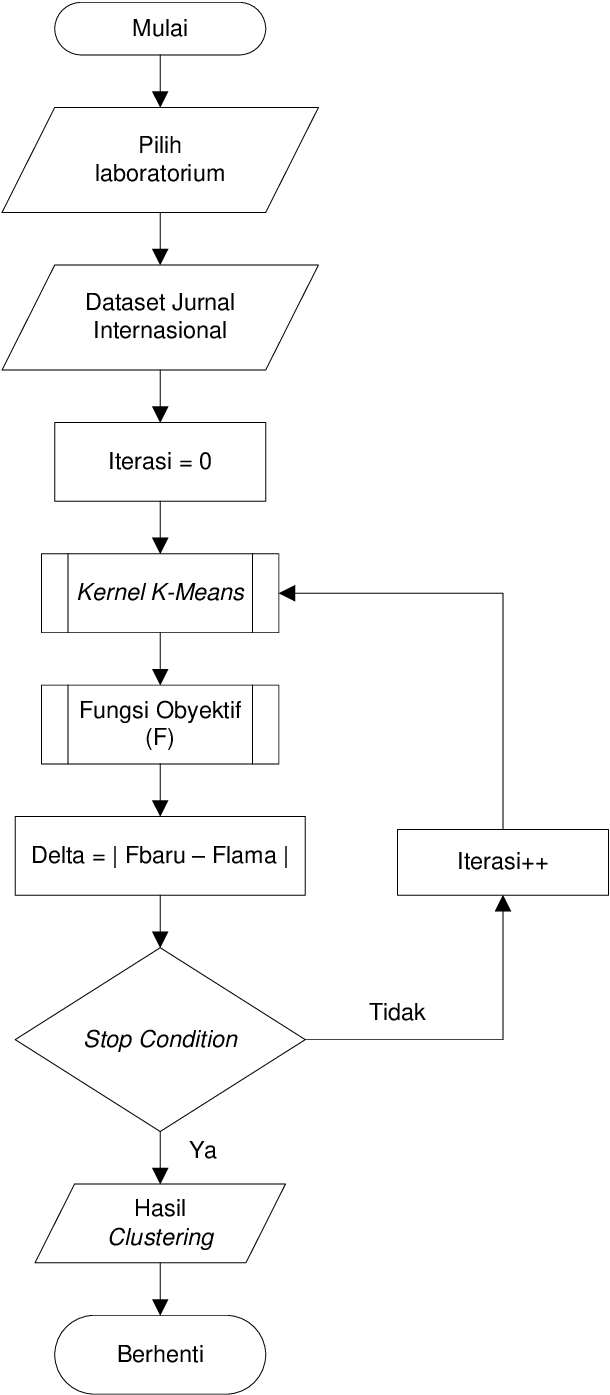
\includegraphics[width=0.40\linewidth]{gambar/flowchart.png}
    \caption{Contoh gambar 2}
    \label{gambar2}
\end{figure}

\section{Alat dan Bahan}
\lipsum[2][4]

\begin{enumerate}
    \item \lipsum[2][5]
    \item \lipsum[2][5]
    \item \lipsum[2][5]
\end{enumerate}

\section{Tahapan Penelitian}
\lipsum[2][4]

\begin{enumerate}
    \item \lipsum[2][5] \\ \lipsum[3]
    \item \lipsum[2][5] \\ \lipsum[3]
    \item \lipsum[2][5] \\ \lipsum[3]
    \item \lipsum[2][5] \\ \lipsum[3]
\end{enumerate}

\section{Perancangan Sistem}
\subsection{Sub Perancangan Sistem I}
\lipsum[2]

\subsection{Sub Perancangan Sistem II}
\lipsum[2]

\begin{table}[H]
    \centering
    \caption{Contoh tabel 2}
    \label{t perbandinganRespon}
    \begin{tabular}{lllll}
        \hline
        \multirow{2}{*}{Karakteristik} & \multicolumn{4}{c}{Perbandingan performa} \\ \cline{2-5} 
        & \multicolumn{1}{c}{\textbf{PID}} & \multicolumn{1}{c}{\textbf{MF3}} & \multicolumn{1}{c}{\textbf{MF5}} & \multicolumn{1}{c}{\textbf{MF7}} \\ \hline
        \textit{Rise time} (s)  & 1,0580  & 1,0740  & 1,0620    & \textbf{1,0450} \\
        \textit{Settling time} (s) & 1,3380 & 1,3410  & 1,3350  & \textbf{1,3290} \\
        \textit{Overshoot} (\%) & 0,0910 & 0,0440  & 0,0593     & \textbf{0,0121} \\
        \textit{Peak} & 1,0910 & 1,0440 & 1,0593 & \textbf{1,0121} \\
        \textit{Peak time} (s) & 1,0840 & 1,3560  & 1,2710      & 1,0520  \\ \hline
    \end{tabular}
\end{table}

\lipsum[2]

\subsection{Sub Perancangan Sistem III}
\lipsum[2]

\subsection{Sub Perancangan Sistem IV}
\lipsum[2]

\section{Pengambilan Data}
\lipsum[2]

\begin{table}[H]
    \centering
    \caption{Contoh tabel 3}
    \label{t bestfits}
    \begin{tabular}{|
        >{\columncolor[HTML]{EFEFEF}}c 
        >{\columncolor[HTML]{C0C0C0}}c |
        >{\columncolor[HTML]{FFFFFF}}c 
        >{\columncolor[HTML]{FFFFFF}}c 
        >{\columncolor[HTML]{FFFFFF}}c 
        >{\columncolor[HTML]{FFFFFF}}c 
        >{\columncolor[HTML]{FFFFFF}}c 
        >{\columncolor[HTML]{FFFFFF}}c |
    }
        \hline
        \multicolumn{2}{|c|}{\cellcolor[HTML]{FFFFFF}{\color[HTML]{000000} }} & \multicolumn{6}{c|}{\cellcolor[HTML]{EFEFEF}\textit{Validation data}} \\ \cline{3-8} 
        \multicolumn{2}{|c|}{\multirow{-2}{*}{\cellcolor[HTML]{FFFFFF}{\color[HTML]{000000} }}} & \multicolumn{1}{c|}{\cellcolor[HTML]{C0C0C0}{\color[HTML]{333333} Data-1}} & \multicolumn{1}{c|}{\cellcolor[HTML]{C0C0C0}{\color[HTML]{333333} Data-2}} & \multicolumn{1}{c|}{\cellcolor[HTML]{C0C0C0}{\color[HTML]{333333} Data-3}} & \multicolumn{1}{c|}{\cellcolor[HTML]{C0C0C0}{\color[HTML]{333333} Data-4}} & \multicolumn{1}{c|}{\cellcolor[HTML]{C0C0C0}{\color[HTML]{333333} Data-5}} & \cellcolor[HTML]{C0C0C0}{\color[HTML]{333333} Data 6} \\ \hline
        \multicolumn{1}{|c|}{\cellcolor[HTML]{EFEFEF}} & {\color[HTML]{333333} $TF_{1}$} & \multicolumn{1}{c|}{\cellcolor[HTML]{FFFFFF}{\color[HTML]{333333} 83,13}} & \multicolumn{1}{c|}{\cellcolor[HTML]{FFFFFF}{\color[HTML]{333333} 77,73}} & \multicolumn{1}{c|}{\cellcolor[HTML]{FFFFFF}{\color[HTML]{333333} 80,74}} & \multicolumn{1}{c|}{\cellcolor[HTML]{FFFFFF}{\color[HTML]{333333} 94,22}} & \multicolumn{1}{c|}{\cellcolor[HTML]{FFFFFF}{\color[HTML]{333333} 85,88}} & {\color[HTML]{333333} 83,76}                         \\ \cline{2-8} 
        \multicolumn{1}{|c|}{\cellcolor[HTML]{EFEFEF}}                                        & {\color[HTML]{333333} $TF_{2}$} & \multicolumn{1}{c|}{\cellcolor[HTML]{FFFFFF}{\color[HTML]{333333} 79,61}} & \multicolumn{1}{c|}{\cellcolor[HTML]{FFFFFF}{\color[HTML]{333333} 83,34}} & \multicolumn{1}{c|}{\cellcolor[HTML]{FFFFFF}{\color[HTML]{333333} 76,93}} & \multicolumn{1}{c|}{\cellcolor[HTML]{FFFFFF}{\color[HTML]{333333} 84,3}} & \multicolumn{1}{c|}{\cellcolor[HTML]{FFFFFF}{\color[HTML]{333333} 82,39}} & {\color[HTML]{333333} 77,31}                         \\ \cline{2-8} 
        \multicolumn{1}{|c|}{\cellcolor[HTML]{EFEFEF}}                                        & {\color[HTML]{333333} $TF_{3}$} & \multicolumn{1}{c|}{\cellcolor[HTML]{FFFFFF}{\color[HTML]{333333} 81,88}}  & \multicolumn{1}{c|}{\cellcolor[HTML]{FFFFFF}{\color[HTML]{333333} 72,91}}  & \multicolumn{1}{c|}{\cellcolor[HTML]{FFFFFF}{\color[HTML]{333333} 82,17}}  & \multicolumn{1}{c|}{\cellcolor[HTML]{FFFFFF}{\color[HTML]{333333} 95,17}}  & \multicolumn{1}{c|}{\cellcolor[HTML]{FFFFFF}{\color[HTML]{333333} 84,9}}  & {\color[HTML]{333333} 81,9}                          \\ \cline{2-8} 
        \multicolumn{1}{|c|}{\cellcolor[HTML]{EFEFEF}}                                        & {\color[HTML]{333333} $TF_{4}$} & \multicolumn{1}{c|}{\cellcolor[HTML]{FFFFFF}{\color[HTML]{333333} 82,6}} & \multicolumn{1}{c|}{\cellcolor[HTML]{FFFFFF}{\color[HTML]{333333} 73,58}} & \multicolumn{1}{c|}{\cellcolor[HTML]{FFFFFF}{\color[HTML]{333333} 81,63}} & \multicolumn{1}{c|}{\cellcolor[HTML]{FFFFFF}{\color[HTML]{333333} 96,21}} & \multicolumn{1}{c|}{\cellcolor[HTML]{FFFFFF}{\color[HTML]{333333} 85,44}} & {\color[HTML]{333333} 84,23}                         \\ \cline{2-8} 
        \multicolumn{1}{|c|}{\cellcolor[HTML]{EFEFEF}}                                        & {\color[HTML]{333333} $TF_{5}$} & \multicolumn{1}{c|}{\cellcolor[HTML]{FFFFFF}{\color[HTML]{333333} 83,13}} & \multicolumn{1}{c|}{\cellcolor[HTML]{FFFFFF}{\color[HTML]{333333} 77,33}} & \multicolumn{1}{c|}{\cellcolor[HTML]{FFFFFF}{\color[HTML]{333333} 80,95}} & \multicolumn{1}{c|}{\cellcolor[HTML]{FFFFFF}{\color[HTML]{333333} 94,59}} & \multicolumn{1}{c|}{\cellcolor[HTML]{FFFFFF}{\color[HTML]{333333} 85,89}} & {\color[HTML]{333333} 83,87}                         \\ \cline{2-8} 
        \multicolumn{1}{|c|}{\multirow{-6}{*}{\cellcolor[HTML]{EFEFEF}\begin{tabular}[c]{@{}c@{}}\rotatebox[origin=c]{90}{\textit{\textit{Transfer function}}}\end{tabular}}} & {\color[HTML]{333333} $TF_{6}$} & \multicolumn{1}{c|}{\cellcolor[HTML]{FFFFFF}{\color[HTML]{333333} 83,56}} & \multicolumn{1}{c|}{\cellcolor[HTML]{FFFFFF}{\color[HTML]{333333} 73,29}} & \multicolumn{1}{c|}{\cellcolor[HTML]{FFFFFF}{\color[HTML]{333333} 81,42}} & \multicolumn{1}{c|}{\cellcolor[HTML]{FFFFFF}{\color[HTML]{333333} 96,17}} & \multicolumn{1}{c|}{\cellcolor[HTML]{FFFFFF}{\color[HTML]{333333} 85,4}} & {\color[HTML]{333333} 84,33}                         \\ \hline
    \end{tabular}
\end{table}

\lipsum[2]

